\documentclass{article}
\usepackage{microtype}
\usepackage[utf8]{inputenc} 
\usepackage[a4paper, total={6in, 9.6in}]{geometry}
\usepackage{MnSymbol}
\usepackage{enumerate}
\usepackage{amsmath}
\usepackage{fancyhdr}
\usepackage{xcolor}
\usepackage{tikz}
\usepackage{pgfplots}
\usepackage{marvosym}

\widowpenalties=4 10000 10000 150 0

%% headers
\pagestyle{fancy}
\fancyhf{}
\rhead{Kommunikationssysteme WS19/20}
\lhead{Daniel Schubert, Anton Lydike}
\rfoot{Seite \thepage}

% simple command to display Aufgabe <num>)       ___ / <num>p.
\newcommand\task[1]{\section*{Aufgabe #1)\hfill \underline{\,\,\,\,\,\,}\,\,/1p.}}

% Interpretation (I)
\newcommand\I{I}
% Interpretation und belegung (I, \beta)
\newcommand\Ib{\I, \beta}

%% models
\newcommand\lmodels{\leftmodels} 			% =|
\newcommand\bimodels{\leftmodels\models}	% =||=


%% table for total points
\newcommand\pointsttl[1]{\section*{Gesamtpunkte: \hfill \underline{\,\,\,\,\,\,}\,\,/#1p.}}

%% Funktionen und Prädikate
% Funktionen (arg ist anzahl der stellen)
\newcommand\func[1]{\mathcal{F}^{#1}}
% Prädikate (arg ist anzahl der stellen)
\newcommand\praed[1]{\mathcal{P}^{#1}}

%% Regeln
\newcommand\defrule[2]{\frac{#1}{#2}}

%% Funktionszahl
\newcommand\funcnum[1]{\#_{F}\, #1}

% Für ersetzungen in belegungen wie { x \mapsto d }
\newcommand\repl[2]{\{#1 \mapsto #2\}}

% für alle x .
\newcommand\fall[1]{\forall #1 \, . \,}
\newcommand\ex[1]{\exists #1 \, . \,}

% short biimplication
\newcommand\biimpl{\Leftrightarrow}

% draw a box on the right side of the page
\newcommand\qed{ \hfill $\Box$ }

% red, green, blue text:

\definecolor{greeen}{RGB}{34,139,34}

\newcommand\red[1]{\textcolor{red}{#1}}
\newcommand\green[1]{\textcolor{greeen}{#1}}
\newcommand\blue[1]{\textcolor{blue}{#1}}

% more symbols: https://oeis.org/wiki/List_of_LaTeX_mathematical_symbols

\newcommand\cfgtitle[1]{\title{\vspace{-1.5cm}Übungsblatt #1\\%
\begin{large} Übungsgruppe Metcalfe \end{large}} \lfoot{Übungsblatt #1}\cfoot{Übungsgruppe Metcalfe}}
\author{Daniel Schubert\\Anton Lydike}


%%%%%%%%%%%%%%%%%%%%%%%
%% plotting helpers  %%
%%%%%%%%%%%%%%%%%%%%%%%

%% these draw vertical features
\newcommand\htl[1]{(#1,1) (#1,-1)}  		%% draw line from low to high
\newcommand\lth[1]{(#1,-1) (#1,1)}			%% draw line from high to low

\newcommand\sigtick[2]{\htl{#1} \lth{#2}}	%% draw a htl and then lth line

%% these draw horizontal features
\newcommand\sig[3]{(#2,#1) (#3,#1)}		%% draw a line at height #1 from x=#2 to x=#3
\newcommand\sighi[2]{\sig{1}{#1}{#2}}		%% draw a high signal from #1 to #2
\newcommand\sigmed[2]{\sig{0}{#1}{#2}}		%% draw a null signal from #1 to #2
\newcommand\siglo[2]{\sig{-1}{#1}{#2}}		%% draw a low  signal from #1 to #2


\newcommand\fakeaxis[2]{\addplot [-stealth,black] coordinates {(#1,0) (#2,0)};}



%% units
\newcommand\m{\text{ m}}
\newcommand\s{\text{ s}}
\newcommand\mps{\frac{\text{m}}{\text{s}}}
\newcommand\Gbps{\text{ Gbps}}
\newcommand\bps{\text{ bps}}
\newcommand\bit{\text{ b}}
\newcommand\B{\text{ B}}


\pgfplotsset{compat=1.15}

\renewcommand{\arraystretch}{1.5}

\newcommand\tunderset[2]{\underset{\text{#1}}{\text{#2}}}

\cfgtitle{11}
\date{Mittwoch 29.1.2020}

\begin{document}
\maketitle
\thispagestyle{fancy}

\task{1}
\begin{enumerate}[a)]
	\item  Die Merkmale der folgenden Vielfachzugriffsverfahren sind: \\
	\begin{tabular}{r|p{13cm}}
		\textit{Verfahren} & \textit{Beschreibung} \\ \hline
		FDMA    & Zuweisung der Kanäle (unterschiedliche Trägerfrequenz, gleichzeitige Übertragung, Kein Qualitätsverlust). \\ \hline
		Polling & Master weist Medium den Stationen zu.\\ \hline
		CSMA    & ,,Zuhören vor dem Sprechen''. 
		Kanal leer $\Rightarrow$ sende Rahmen.
		Kanal besetzt $\Rightarrow$ Übertragung verschieben.
		Kollision $\Rightarrow$ zufälligen Zeitspanne warten, dann wie oben. \\ 
	\end{tabular}
	\item { \hfill \\
	\begin{tabular}{p{11.2cm}cc}
													& Korrekt & Falsch \\
		Das Slotted ALOHA erfordert, dass alle Knoten ihre Übertragungen syn-
		chronisieren								& $\bigotimes$   & $\bigcirc$ \\ \\
		CSMA verringert die Kollisionswahrscheinlichkeit gegenüber ALOHA
													& $\bigotimes$   & $\bigcirc$ \\ \\
		Beim 1-persistenten CSMA wird ein Rahmen übertragen, wenn die Station
		einen freien Kanal vorfindet				& $\bigotimes$   & $\bigcirc$     
	\end{tabular}}
	\item \begin{itemize}
		\item Die wahrscheinlichkeit beträgt $p\cdot(1-p)^{N-1}$
		\item $p^*= \,\,???$
	\end{itemize}
\end{enumerate}

\pagebreak

\task{2}
\begin{enumerate}[a)]
	\item $d_{AB} = d_{BC} = 400m, R= 100Mbps, v_s=2*10^8m/s$
		\begin{itemize}
			\item \hfill \begin{center}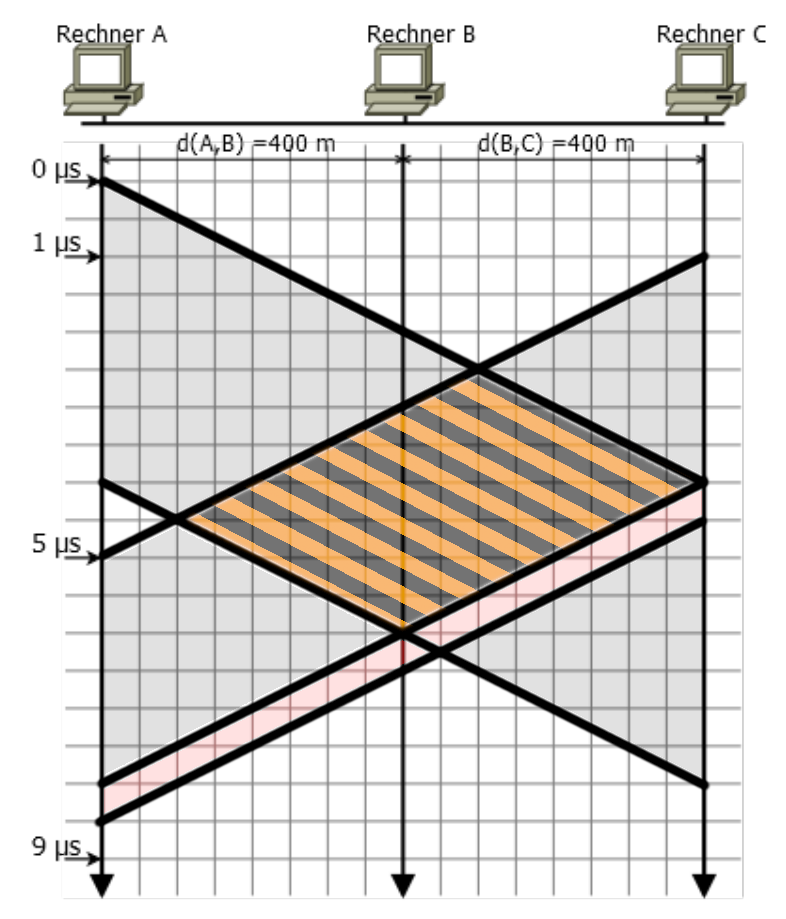
\includegraphics[]{2a.png}\end{center}
			\item Rechner B Bekommt "bad data", aber das "Jam-Signal", kommt erst nach vollendeter übertragung an.
			\item $L_{min} > 100Mb$
		\end{itemize}
	\item Der \emph{binare exponentielle Backoff-Algorithmus} verringert die wahrscheinlichkeit einer erneuten Kollision, da beide parteien unterschiedlich lange warten, bis sie erneut senden.
	\item Die Folgenden Felder befinden sich in einem Ethernet Frame: \\
	\begin{tabular}{p{11.2cm}cc}
												& Ja           & Nein \\
		Quelle-MAC-Adresse						& $\bigotimes$ & $\bigcirc$ \\
		Time-to-Live bzw. Hop Count				& $\bigcirc$   & $\bigotimes$ \\
		Sequenznummer							& $\bigcirc$   & $\bigotimes$ \\
		CRC-Prüfsumme							& $\bigotimes$ & $\bigcirc$     
	\end{tabular}
\end{enumerate}

\task{3}
\begin{enumerate}[a)]
	\item {\hfill\\
	\begin{tabular}{p{11.2cm}cc}
											& Richtig     & Falsch \\
	Switches sind für die angeschlossenen Stationen transparent		& $\bigotimes$ & $\bigcirc$ \\
	Der Spanning-Tree-Algorithmus wird erst angewendet, wenn die Switchtabellen erzeugt wurden		& $\bigotimes$   & $\bigcirc$ \\
	Am Ende des Spanning-Tree-Protokolls soll jeder Switch ein eigenen Designated Port bestimmen		& $\bigcirc$   & $\bigotimes$
	\end{tabular}}
	
	\item {\hfill \\ 
	\begin{center}
		\begin{tabular} {l||l|l||l|l||l|l}
			      & \multicolumn{2}{c||}{Switch S1} & \multicolumn{2}{c||}{Switch S2} & \multicolumn{2}{c}{Switch S3} \\
			      & Port & Mac-Adresse & Port & Mac-Adresse & Port & Mac-Adresse \\ \hline
		1) A $\to$ B & 3    & MAC A       & 3	  & MAC A       & 1    & MAC A       \\ \hline
		2) A $\to$ D & -    & -           & -	  & -           & -    & -           \\ \hline
		3) C $\to$ A & 1    & MAC C       & 2	  & MAC C       & 3    & MAC C       \\ 
		\end{tabular}
	\end{center}

	\begin{itemize}
		\item Rahmen 1) und 2) kommen bei allen Hosts an. 
		\item Rahmen 3) geht S3$\to$S2$\to$S1$\to$Host A.
	\end{itemize}
	}
	
	\item Da das Netz hier nicht Zyklus-Frei ist, werden Pakete unendlich lange weitergeleitet. Das führt dazu, dass Informationen in den Routing-Tabellen nutzlos sind. 

	\item {\hfill \\ \begin{tabular}{lclccc}
		\emph{Switch} & \emph{Root-Switch?} & \emph{Ports} & \emph{Root-Port?} & \emph{Designated-Port?} & \emph{Blocking-Port?} \\ \hline 
		Switch 1	  & $\bigotimes$        & P1           & $\bigcirc$        & $\bigotimes$            & $\bigcirc$            \\
					  &                     & P2           & $\bigcirc$        & $\bigotimes$            & $\bigcirc$            \\ \hline 
		Switch 2	  & $\bigcirc$          & P1           & $\bigcirc$        & $\bigcirc$              & $\bigotimes$          \\
			          &                     & P2           & $\bigcirc$        & $\bigotimes$            & $\bigcirc$            \\ 
					  &                     & P3           & $\bigotimes$      & $\bigcirc$              & $\bigcirc$            \\ \hline
		Switch 3	  & $\bigcirc$          & P1           & $\bigcirc$        & $\bigotimes$            & $\bigcirc$            \\
			          &                     & P2           & $\bigcirc$        & $\bigotimes$            & $\bigcirc$            \\ 
			          &                     & P3           & $\bigotimes$      & $\bigcirc$              & $\bigcirc$            \\ \hline
		Switch 4	  & $\bigcirc$          & P1           & $\bigcirc$        & $\bigcirc$              & $\bigotimes$          \\
			          &                     & P2           & $\bigotimes$      & $\bigcirc$              & $\bigcirc$            \\ 
			          &                     & P3           & $\bigcirc$        & $\bigcirc$              & $\bigotimes$          \\ 
			          &                     & P4           & $\bigcirc$        & $\bigotimes$            & $\bigcirc$            \\ \hline
		Switch 5	  & $\bigcirc$          & P1           & $\bigotimes$      & $\bigcirc$              & $\bigcirc$            \\
			          &                     & P2           & $\bigcirc$        & $\bigcirc$              & $\bigotimes$          \\ \hline
		Switch 6	  & $\bigcirc$          & P1           & $\bigotimes$      & $\bigcirc$              & $\bigcirc$            \\
			          &                     & P2           & $\bigcirc$        & $\bigcirc$              & $\bigotimes$          \\ \hline

	\end{tabular}}
	
\end{enumerate}

\pointsttl{3}
\end{document}